\documentclass{article}
\usepackage{xr}
\usepackage{graphicx} % Para incluir imágenes
\usepackage[spanish]{babel}
\usepackage{makeidx}
\usepackage{geometry}
\usepackage{amsmath}
\usepackage{graphicx}
\usepackage{caption}
\usepackage{pdfpages}
\usepackage{hyperref}
\usepackage{placeins}
\usepackage{adjustbox}

\hypersetup{
    colorlinks,
    citecolor=black,
    filecolor=black,
    linkcolor=black,
    urlcolor=black
}



\geometry{a4paper, total={170mm,257mm}, left=20mm, top=20mm}
\renewcommand{\familydefault}{\sfdefault}


\begin{document}
\begin{titlepage}
    \centering
    \Large
    Universidad Central de Venezuela\\
    Facultad de Ingeniería\\
    Escuela de Ingeniería Eléctrica
    \vspace*{8cm}

    \Huge
    \textbf{Prelaboratorio N° 11: } 

    \textbf{Multivibradores}
    \vfill


    \Large

    Emerson Warhman \\
    C.I. 25.795.480 \\
    \today

\end{titlepage}
\tableofcontents
\newpage

\section{Objetivos}


\begin{itemize}
    \item Reconocer, comprender y utilizar algunas de las aplicaciones del amplificador operacional más frecuentemente utilizadas
\end{itemize}

\section{Marco Teórico}

\subsection{Filtros activos}

Un filtro es en general aquel dispositivo que modifica linealmente el
contenido espectral de una señal. Un filtro activo es aquel el cual, ademas de contar con elementos pasivos, también tiene elementos activos cómo el amplificador operacional.

No es difícil encontrar una situación cuyos requerimientos exijan un filtro de orden alto y tampoco es imposible realizarlo, lo difícil es sintonizarlo, esto es, hacer que cada coeficiente de la función de transferencia tome el valor adecuado para cumplir con los requerimientos.

La sintonización se hace difícil, porque los parámetros de red susceptibles de variarse, modifican a mas de un coeficiente a la vez y si el número de coeficientes es alto, la tarea, además de ser iterativa, es muy costosa en tiempo y en equipos.

Si el orden del filtro es alto, entonces puede dividirse en una cascada de etapas de 2do orden y a lo mas una de primer orden en el caso de orden impar

\begin{align*}
    H &= \frac{1}{s^5 + 3.236s^4 + 5.236s^3 + 5.236s^2 + 3.236s + 1} \\
    H &= \frac{1}{(s^2 + 0.61803s + 1) \cdot (s^2 + 1.61803) \cdot (s + 1)}
\end{align*}

De manera tal que solo sea necesario sintonizar varias etapas de 2do orden y quizás de 1er orden, que aunque para cada una de ellas debe sintonizarse iterativamente, llevarán mucho menor tiempo y con la garantía de convergencia.

\subsubsection{Función de transferencia de los filtros}

Las funciones de transferencia de los filtros más utilizados son bien conocidas y son las siguientes:

\begin{itemize}
\item 
Pasa bajos:
\begin{multicols}{2}
\begin{equation}
    H(s) = \frac{H_o \cdot \omega_o^2}{s^2 + \alpha \cdot \omega_o \cdot s + \omega_o^2}
    \label{eq:func-transferencia-pasa-bajos}
\end{equation}
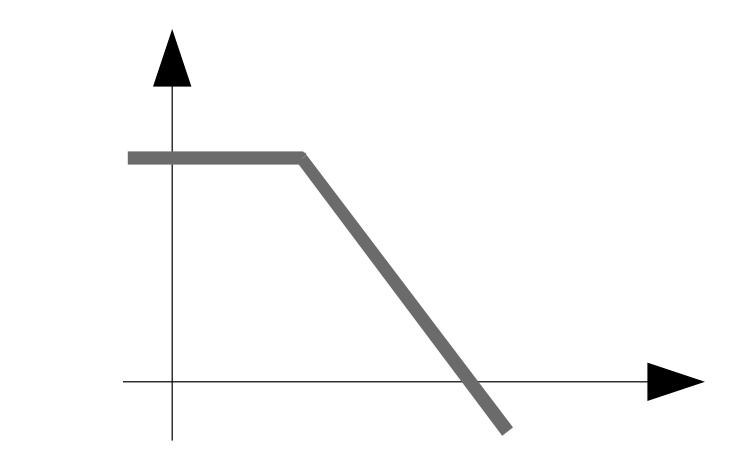
\includegraphics[width=0.1\textwidth]{marco-teorico/respuesta-freq-pasa-bajos.png}
\end{multicols}
    \item 
    Pasa banda:
    \begin{multicols}{2}
    \begin{equation}
        H(s) = \frac{H_o \cdot \omega_o \cdot s}{s^2 + \alpha \cdot \omega_o \cdot s + \omega_o^2}
        \label{eq:func-transferencia-pasa-banda}
    \end{equation}
    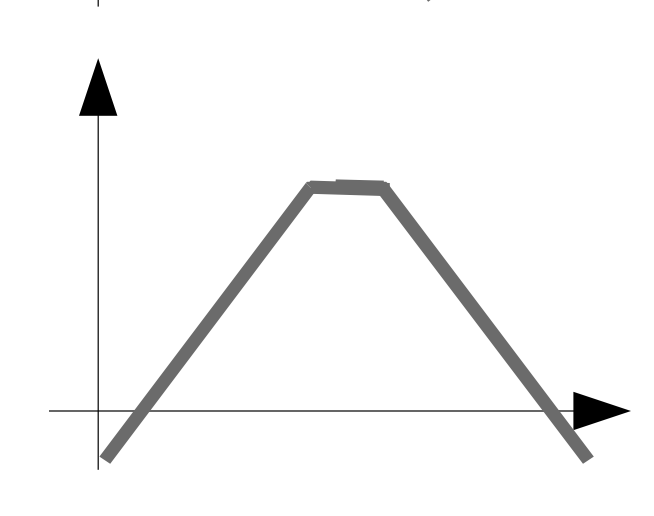
\includegraphics[width=0.1\textwidth]{marco-teorico/respuesta-freq-pasa-banda.png}
    \end{multicols}
Pasa altos:
\begin{multicols}{2}
\begin{equation}
    H(s) = \frac{H_o \cdot s^2}{s^2 + \alpha \cdot \omega_o \cdot s + \omega_o^2}
    \label{eq:func-transferencia-pasa-altos}
\end{equation}
    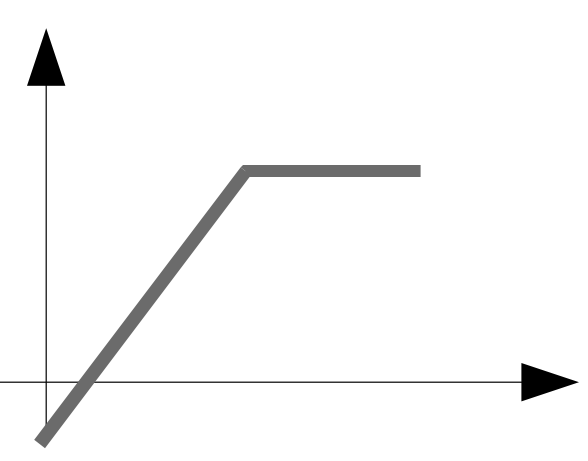
\includegraphics[width=0.1\textwidth]{marco-teorico/respuesta-freq-pasa-altos.png}
\end{multicols}
Rechaza banda:
\begin{multicols}{2}
\begin{equation}
    H(s) = \frac{H_o \left( s^2 + \omega_o^2 \right)}{s^2 + \alpha \cdot \omega_o \cdot s + \omega_o^2}
    \label{eq:func-transferencia-rechaza-banda}
\end{equation}
    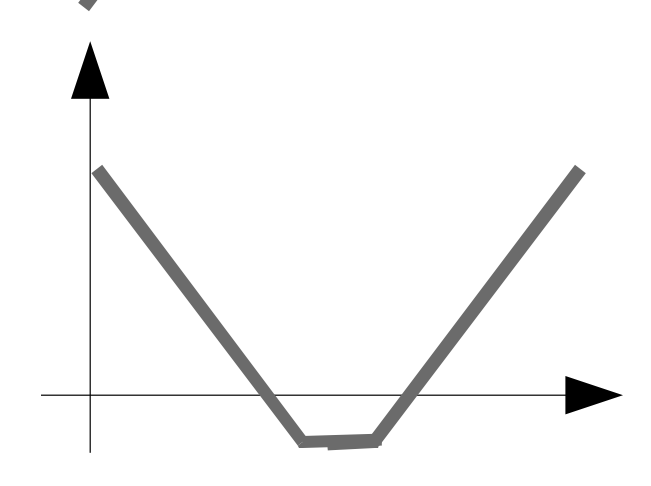
\includegraphics[width=0.1\textwidth]{marco-teorico/respuesta-freq-rechaza-banda.png}
\end{multicols}
\end{itemize}

\subsection{Filtros de múltiples realimentaciones}

Esta topología puede convertirse en un cualquiera de las funciones de segundo orden (pasa bajo, pasa alto o pasa banda) con solo ubicar apropiadamente resistencias y condensadores.

\begin{figure}[ht]
    \centering
    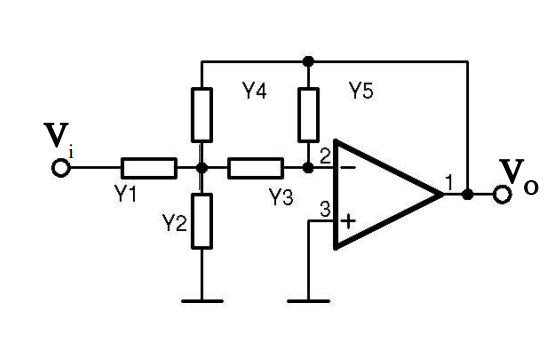
\includegraphics[width=0.5\textwidth]{marco-teorico/filtro-multiples-realimentaciones.png}
    \caption{Filtro de múltiples realimentaciones}
    \label{fig:filtro-multiples-realimentacion}
\end{figure}

La función de transferencia puede resolverse de varias maneras, pero resulta compacto en términos de sus admitancias y usando el inversor $-Y_3/Y_5$ como amplificador base.

Utilizando el método del amplificador desvanecido, tenemos:

$$A_b = - \frac{Y_3}{Y_5}$$

\begin{align*}
    a_{io} &= 0 \\
    a_{i1} &= \frac{Y_1}{Y_1 + Y_2 + Y_3 + Y_4}\\
    a_{31} &= \frac{Y_4}{Y_1 + Y_2 + Y_3 + Y_4}\\
    a_{3o} &= 1
\end{align*}

Aplicandolo a la formula MAD:

\begin{equation}
    \frac{V_o}{V_i} = \frac{Y_1}{Y_1 + Y_2 + Y_3 + Y_4} \frac{\frac{-Y_3}{Y_5}}{1 - \frac{Y_4}{Y_1 + Y_2 + Y_3 + Y_4} \WrapParenthesis{\frac{-Y_3}{Y_5}}}
\end{equation}

lo cual queda como:

\begin{equation}
    \frac{V_o}{V_i} = \frac{-Y_1 \cdot Y_3}{Y_5(Y_1 + Y_2 + Y_3 + Y_4)+ Y_3.Y_4} 
    \label{eq:filtro-multirealimentacion}
\end{equation}

\subsubsection{Filtro pasa bajo de múltiples realimentaciones}

\begin{figure}[ht]
    \centering
    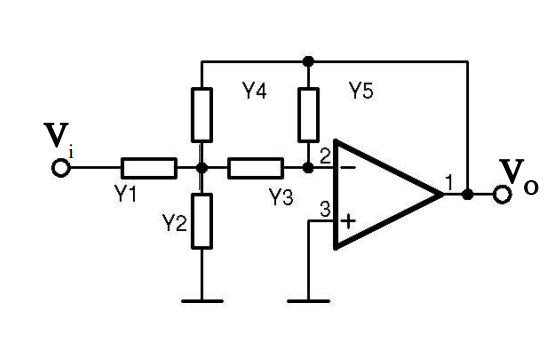
\includegraphics[width=0.5\textwidth]{marco-teorico/filtro-multiples-realimentaciones.png}
    \caption{Filtro pasa bajo de múltiples realimentaciones}
    \label{fig:filtro-multiples-realimentacion-pasa-bajo}
\end{figure}

Al sustituir las admitancias $Y_2$ y $Y_5$ de la figura \ref{fig:filtro-multiples-realimentacion} por condensadores, obtenemos un filtro pasa bajo con la siguiente función de transferencia:

\begin{equation}[ht]
    H(s) = \frac{V_o(s)}{V_i(s)} = \frac{-\frac{1}{R_1}\cdot R_2C_2 C_5}{s^2 + (1/C_2)(1/R_1 + 1/R_3 + 1/R_4)s + 1/(R_3 R_4 C_2 C_5)}
    \label{eq:func-transferencia-pasa-bajos-multirealimentacion}
\end{equation}

\subsection{Filtro por fuente de tensión controlada por tensión o Sallen-Key}

Usando esta estructura y ubicando en ella solo capacitancias y resistencias (sin inductancias) pueden lograrse los tres tipos de filtro básicos, esta vez, sin inversión de fase.

\begin{figure}[ht]
    \centering
    \includegraphics[width=0.5\textwidth]{marco-teorico/filtro-sallen-key.png}
    \caption{Filtro con topología de Sallen-Key}
    \label{fig:filtro-activo-sallen-key}
\end{figure}

Tomando en cuenta que:

\begin{equation}
    K = 1 + \frac{R_B}{R_A}
\end{equation}

Aplicando el método del amplificador desvanecido, tenemos:

\begin{align}
    A &= K \\
    a_{io} &= 0 \\
    a_{i1} &= \frac{Y_1}{Y_1 + Y_2 + Y_3 + \WrapParenthesis{\frac{Y_4 Y_5}{Y_4}} + Y_5} \WrapParenthesis{\frac{Y_4}{Y_4 + Y_5}} \\
    a_{30} &= 1 \\
    a_{31} &= \frac{Y_2}{Y_1 + Y_2 + Y_3 + \WrapParenthesis{\frac{Y_4 Y_5}{Y_4 + Y_5}}} \WrapParenthesis{\frac{Y_4}{Y_4 + Y_5}} \\
\end{align}

Sustituyendo en la ecuación MAD:

\begin{equation}
    H(s) = \frac{V_o}{V_i} = \frac{Y_1 Y_4 K}{(Y_1 + Y_2 * Y_3 + Y_4)Y_5 + (Y_1 +Y_2(1-K)+Y_3)Y_4}
\end{equation}

\subsubsection{Filtro pasa bajo de topología de Sallen-Key}

sustituyendo $Y_2$ y $Y_5$ por condensadores, obtenemos un filtro pasa bajo con la siguiente función de transferencia:


\begin{figure}
    \centering
    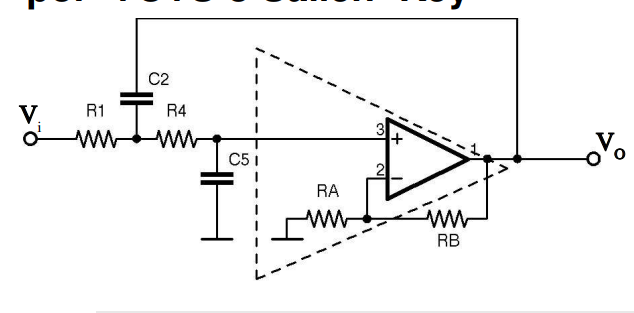
\includegraphics[width=0.5\textwidth]{marco-teorico/filtro-pasa-bajo-sallen-key.png}
    \caption{Filtro pasa bajo de topología de Sallen-Key}
\end{figure}

Al sustituir las admitancias $Y_2$ y $Y_5$ de la figura \ref{fig:filtro-activo-sallen-key} por condensadores, obtenemos un filtro pasa bajo con la siguiente función de transferencia:

\begin{equation}
    H(s) = \frac{\frac{K}{R_1 R_4 C_2 C_5}}{s^2 + \left(\frac{1}{R_1 C_2} + \frac{1}{R_4 C_2} + \left(1 - K\right) \frac{1}{R_4 C_5}\right)s + \frac{1}{R_1 R_4 C_2 C_5}}
    \label{eq:transferencia-pasa-bajo-sallen-key}
\end{equation}

\section{Trabajo de preparación}

Para cada uno de los circuitos que se muestran en las figuras \ref{fig:filtro-variables-de-estado}, \ref{fig:filtro-sallen-key} y \ref{fig:filtro-realimentacion-multiple}, se debe realizar el siguiente proceso de preparación:

\begin{enumerate}
    \item Obtener su modelo circuital de entrada a cada una de sus salidas, observar la importancia de la función de transferencia.
    \item Especificar los componentes necesarios, en cada filtro, para obtener frecuencias de corte de $2.7 kHz$ con factor de amortiguamiento de 0.707, con ganancia de 2 en la salida pasa bajos.
    \item Verificar sus diseños, mediante simulación, comparando la respuesta en frecuencia obtenida, con el diagrama asintótico de Bode de cada filtro. Determine la ganancia de cada filtro a las frecuencias en las que planea medir la respuesta en frecuencia.
    \item Por simulación obtener las formas en cada salida al inyectar señales cuadradas con frecuencia tal, que su tercera armónica, coincida con la frecuencia de corte indicadas. Explicar a que se deben las formas de onda obtenidas.
    \item Elabore la hoja de datos necesaria para recabar las mediciones y los datos del montaje, en los ensayos descritos por usted previamente.
\end{enumerate}

\begin{figure}[ht]
    \centering
    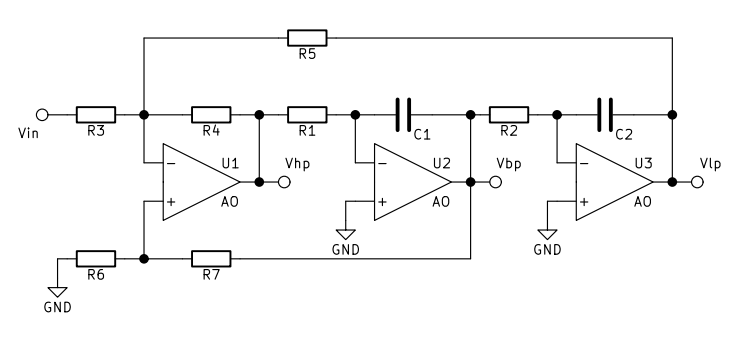
\includegraphics[width=0.8\textwidth]{filtro-variables-de-estado.png}
    \caption{Filtro de variables de estado}
    \label{fig:filtro-variables-de-estado}
\end{figure}

\begin{figure}[ht]
    \centering
    \includegraphics[width=0.6\textwidth]{filtro-sallen-key.png}
    \caption{Filtro pasa bajos con topología de Sallen-Key}
    \label{fig:filtro-sallen-key}
\end{figure}

\begin{figure}[ht]
    \centering
    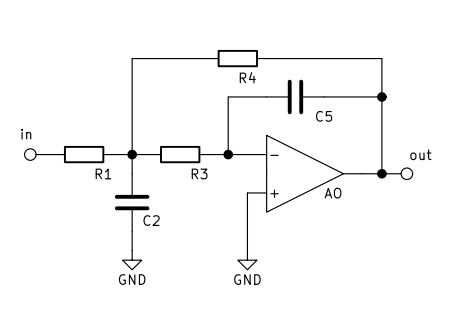
\includegraphics[width=0.5\textwidth]{filtro-realimentacion-multiple.png}
    \caption{Filtro pasa bajos con realimentación múltiple}
    \label{fig:filtro-realimentacion-multiple}
\end{figure}

\FloatBarrier
\subsubsection{Filtro de variables de estado}

De la figura \ref{fig:filtro-variables-de-estado} se observa que las etapas con los amplificadores $U2A0$ y $U3A0$ corresponden a a integradores con ganancia $A = \frac{1}{RCs}$, por lo tanto podemos expresar $V_{bp}$ y $V_{lp}$ como:

\begin{equation}
    \VLP = \frac{1}{R_2 C_2 s}V_{bp}
    \label{eq:vo-integrador-2}
\end{equation}

\begin{equation}
    \VBP = \frac{1}{R_1 C_1 s}V_{hp}
    \label{eq:vo-integrador-1}
\end{equation}

El amplificador $U1A0$ recibe las señales $V_{in}$, $V_{BP}$ y $V_{R6}$, teniendo en cuenta que la caída de tensión en $R_6$ es:

$$V_{R6} = \frac{R_6}{R_6 + R_7}\VBP$$

podemos expresar la tensión $\VHP$ cómo:

\begin{equation}
    \VHP = -\frac{R_4}{R_3}\VIN -\frac{R_4}{R_5}\VLP + \left (1 + \frac{R_4}{R_3 \parallel R_5}\right )\frac{R_6}{R_6 + R_7}\VBP
    \label{eq:vhp-uno}
\end{equation}

Ahora, usando las ecuaciones \ref{eq:vo-integrador-1} y \ref{eq:vo-integrador-2} podemos expresar la tensión de salida $\VBP$ cómo:

\begin{equation}
    \VLP = \frac{1}{R_2 C_2 s} \frac{1}{R_1 C_1 s}\VHP
    \label{eq:vlp-ambos-integradores}
\end{equation}

Sustituyendo la ecuación \ref{eq:vo-integrador-1} en la ecuación \ref{eq:vhp-uno} obtenemos:

\begin{equation}
    \VHP = -\frac{R_4}{R_3}\VIN -\frac{R_4}{R_5}\VLP + \WrapParenthesis{1 + \frac{R_4}{R_3 \parallel R_5}}\frac{1}{R_1 C_1 s}\frac{1}{R_2 C_2 s}\frac{R_6}{R_6 + R_7}\VHP
    \label{eq:vhp-dos}
\end{equation}

Despejando $\VHP$:

\newcommand{\VHPEq}{
    - \frac{\frac{R_4}{R_3}\VIN + \frac{R_4}{R_5}\VLP}{1 + \frac{R_6}{R_6 + R_7} \WrapParenthesis{1 + \frac{R_4}{R_3 \parallel R_5}}\frac{1}{R_1 C_1 s}}
}
\newcommand{\Numerador}{\frac{R_4}{R_3}\VIN + \frac{R_4}{R_5}\VLP}

\newcommand{\Denominador}{1 + \frac{R_6}{R_6 + R_7} \WrapParenthesis{1 + \frac{R_4}{R_3 \parallel R_5}}\frac{1}{R_1 C_1 s}}



\begin{equation}
    \VHP = \VHPEq
    \label{eq:vhp-tres}
\end{equation}

De la ecuación \ref{eq:vhp-tres} podemos definir el denominador como $D_1$:

\begin{equation}
    D_1 = \Denominador
    \label{eq:d1}
\end{equation}



Sustituyendo la ecuación \ref{eq:vhp-tres} en la ecuación \ref{eq:vlp-ambos-integradores} obtenemos:

\begin{equation}
    \VLP = - \frac{1}{R_2 C_2 s} \frac{1}{R_1 C_1 s}\WrapParenthesis{\frac{\Numerador}{D_1}}
    \label{eq:vlp-ambos-integradores-sustituido}
\end{equation}

Despejando $\VLP / \VIN$, tenemos:

\begin{equation}
    \frac{\VLP}{\VIN} = - \frac{\frac{1}{R_2 C_2 s} \frac{1}{R_1 C_1 s} \frac{R_4}{R_3} \cancel{\frac{1}{D_1}}}{\WrapParenthesis{D_1 +\frac{1}{R_2 C_2 s} \frac{1}{R_1 C_1 s} \frac{R_4}{R_5}} \cancel{\frac{1}{D_1}}}
\end{equation}

Cancelando $\frac{1}{D_1}$:

\begin{equation}
    \frac{\VLP}{\VIN} = - \frac{\cancel{\frac{1}{R_2 C_2 s}} \cancel{\frac{1}{R_1 C_1 s}} \frac{R_4}{R_3}}{\WrapParenthesis{D_1 R_2 C_2 R_1 C_1 s^2 + \frac{R_4}{R_5}}\cancel{\frac{1}{R_2 C_2 s}} \cancel{\frac{1}{R_1 C_1 s}}}
\end{equation}

Cancelando $\frac{1}{R_2 C_2 s} y \frac{1}{R_1 C_1 s}$ tenemos:

\begin{equation}
    \frac{\VLP}{\VIN} = - \frac{R_4}{R_3}\frac{1}{\WrapParenthesis{D_1 R_2 C_2 R_1 C_1 s^2 + \frac{R_4}{R_5}}}
    \label{eq:vlp-vin-uno}
\end{equation}

Ahora, sustituyendo $D_1$ (ecuación \ref{eq:d1}) en \ref{eq:vlp-vin-uno} obtenemos:

\begin{equation}
    \frac{\VLP}{\VIN} = - \frac{R_4}{R_3}\frac{1}{\WrapParenthesis{\WrapBrackets{\Denominador} R_2 C_2 R_1 C_1 s^2 + \frac{R_4}{R_5}}}
    \label{eq:vlp-vin-dos}
\end{equation}

Por simplificación podemos decir que:

\begin{align*}
    R_1 = R_2 \\
    C_1 = C_2
\end{align*}

Por lo tanto, podemos reescribir la ecuación \ref{eq:vlp-vin-dos} como:


\begin{equation}
    \frac{\VLP}{\VIN} = - \frac{R_4}{R_3 R_1^2 C_1^2} \frac{1}{s^2 + s \frac{R_6}{R_6 + R_7} \frac{R_3 \parallel R_5 + R_4}{R_3 \parallel R_5} \frac{1}{C_1 R_1} + \frac{R_4}{R_5 R_1^2 C_1^2}}
\end{equation}

Usando la formula de filtros pasa bajos, tenemos:

\begin{align}
    \freqCorte^2 &= \frac{R_4}{R_5 R_1^2 C_1^2} \label{eq:freq-corte-variable-de-estado} \\
    \howoSQT &= - \frac{R_4}{R_3 R_1^2 C_1^2} \label{eq:howo-sqt-variable-de-estado} \\
    \gananciaFiltro &= -\frac{R_5}{R_3} \label{eq:ganancia-filtro-variable-de-estado}
\end{align}

\begin{equation}
    2\factorAmortiguamiento\freqCorte = \frac{R_6}{R_6 + R_7} \frac{R_3 \parallel R_5 + R_4}{R_3 \parallel R_5} \frac{1}{C_1 R_1} 
    \label{eq:factor-amortiguamiento-variable-de-estado}
\end{equation}

Sustituyendo los valores deseados tenemos:
\begin{align*}
    \gananciaFiltro &= -2 = -\frac{R_5}{R_3} \\
    R_5 &= 2 R_3 \\
\end{align*}

por lo tanto:

$$ R_3 \parallel R_5 = R_3 \parallel 2 R_3 = \frac{2}{3}R_3 $$

ahora, en primer lugar escogeremos un valor para $C_1$ ya que es el componente que menor opciones tiene:

\begin{equation*}
    \boxed{C_1 = 10 nF}
\end{equation*}

por simplificación diremos que $R_5 = R_4$, por tanto:

\begin{equation}
    \freqCorte = \frac{1}{R_1 C_1}
\end{equation}

de este modo, partiendo de la ecuación \ref{eq:freq-corte-variable-de-estado} obtenemos:

\begin{align*}
    R_1 &= \frac{1}{\freqCorte C_1} \\
    R_1 &= \frac{1}{2\pi 2.7\times 10^3 \cdot 10\times 10^{-9}} \\
\end{align*}
\begin{equation}
    \boxed{R_1 = R_2 = 5894 \Omega}
\end{equation}

Ahora, partiendo de la ecuación \ref{eq:factor-amortiguamiento-variable-de-estado} y tomando en cuenta que $R_4 = R_5 = 2 R_3$ tenemos:

\begin{align*}
    2\factorAmortiguamiento &= \frac{R_6}{R_6 + R_7} \WrapParenthesis{\frac{\frac{2}{3} R_3 + 2R_3}{\frac{2}{3} R_3}} \\
    2\factorAmortiguamiento &= \frac{R_6}{R_6 + R_7} \cdot 4  \\
    \factorAmortiguamiento &= \frac{R_6}{R_6 + R_7} \cdot 2 \\
\end{align*}

Despejando $R_7$:

\begin{align*}
    R_7 &= \WrapParenthesis{\frac{2}{\factorAmortiguamiento} - 1}R_6 \\
\end{align*}

Haciendo
 $$\boxed{R_6 = 10k\Omega}$$
 
tenemos:
\begin{align*}
    R_7 &= \WrapParenthesis{\frac{2}{0.707} - 1} 10\times 10^{3} \\
\end{align*}
\begin{equation}
    \boxed{R_7 = 18288\Omega}
\end{equation}

Por último, si decimos que:

$$\boxed{R_3 = 1k\Omega}$$

entonces:

\begin{equation*}
    \boxed{R_4 = R_5 = 2k\Omega}
\end{equation*}


\begin{figure}[ht]
    \centering
    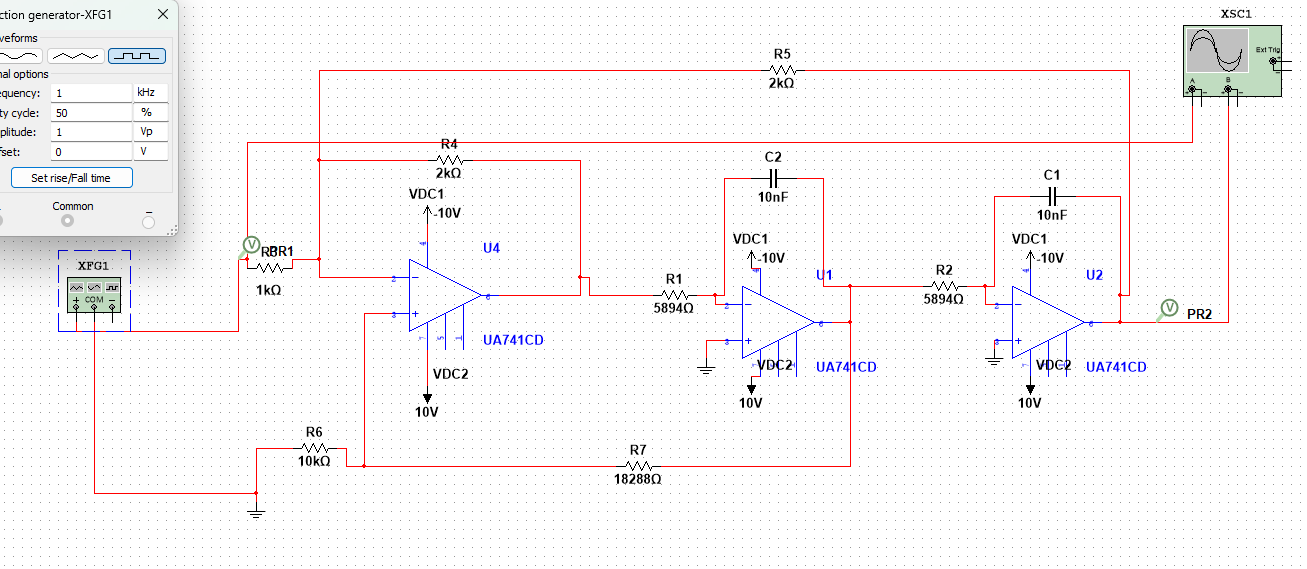
\includegraphics[width=0.8\textwidth]{simulaciones/variables-montaje.png}
    \caption{Montaje Filtro variables de estado}\label{fig:sim-variables-montaje} 
\end{figure}

\begin{figure}[ht]
    \centering
    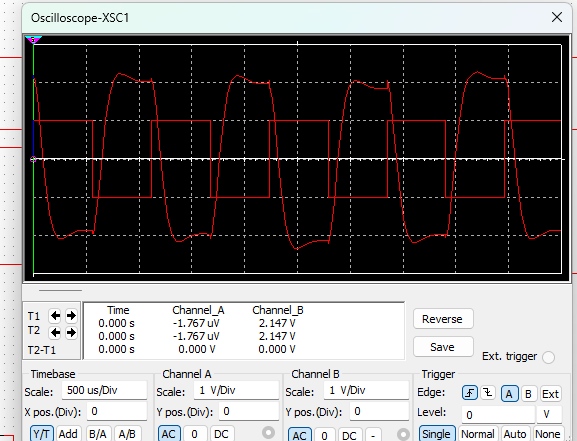
\includegraphics[width=0.8\textwidth]{simulaciones/variables-cuadrada.png}
    \caption{Filtro variables de estado respuesta a onda cuadrada  }
    \label{fig:sim-variables-cuadrada} 
\end{figure}

\begin{figure}[ht]
    \centering
    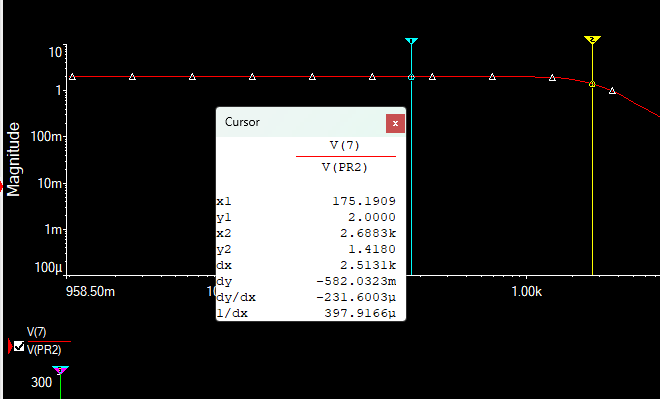
\includegraphics[width=0.8\textwidth]{simulaciones/variables-respuesta.png}
    \caption{Filtro variables de estado respuesta en frecuencia  }
\end{figure}

\FloatBarrier
\subsubsection{Filtro pasa bajos con topología de Sallen-Key}

Para diseñar este filtro partimos de la ecuación \ref{eq:transferencia-pasa-bajo-sallen-key} de la función de transferencia de un filtro pasa bajos con topología de Sallen-Key.

Para la ganancia del filtro, tenemos:

\begin{equation*}
    \gananciaFiltro = K = 2
\end{equation*}

Tenemos:

\begin{equation}
    K = 1 + \frac{R_B}{R_A}
\end{equation}

por tanto:

\begin{align*}
    2 = 1 + \frac{R_B}{R_A}
    1 = \frac{R_B}{R_A}
\end{align*}

\begin{equation*}
    \boxed{R_B = R_A}
\end{equation*}

a estas resistencias les pondremos el valor:

\begin{equation*}
    \boxed{R_B = R_A = 10k\Omega}
\end{equation*}

Ahora seleccionamos los condensadores, por simplicidad podemos hacer

\begin{equation*}
    \boxed{C_2 = C_5 = 10nF}
\end{equation*}

de la función de transferencia obtenemos:

\begin{equation}
    2\factorAmortiguamiento \freqCorte = \left(\frac{1}{R_1 C_2} + \frac{1}{R_4 C_2} + \left(1 - K\right) \frac{1}{R_4 C_5}\right)
\end{equation}

Teniendo en cuenta $C_2 = C_5$ y $K=2$ tenemos:

\begin{equation}
    2\factorAmortiguamiento \freqCorte = \frac{1}{R_1 C_2}
\end{equation}

\begin{align*}
    R_1 &= \frac{1}{2\factorAmortiguamiento \freqCorte C_2} \\
    R_1 &= \frac{1}{2 (0.707) \cdot 2\pi 2.7\times 10^3 \cdot 10\times 10 ^{-9}}
\end{align*}

\begin{equation*}
    R_1 = 4168.76 \Omega
\end{equation*}

Ahora para encontrar $R_2$ tenemos que:

\begin{equation}
    \freqCorte^2 = \frac{1}{R_1 C_1 R_2 C_2} = \frac{1}{R_1 R_2 C_1^2}
\end{equation}

despejando $R_2$ tenemos:

\begin{align*}
    R_2 &= \frac{1}{\freqCorte^2 C_1^2 R_1} \\
    R_2 &= \frac{1}{(2\pi 2.7\times 10^3 \cdot 10\times 10^{-9})^2 \cdot 4168} \\
\end{align*}

\begin{equation*}
    \boxed{R_2 = 8335 \Omega}
\end{equation*}

\begin{figure}[ht]
    \centering
    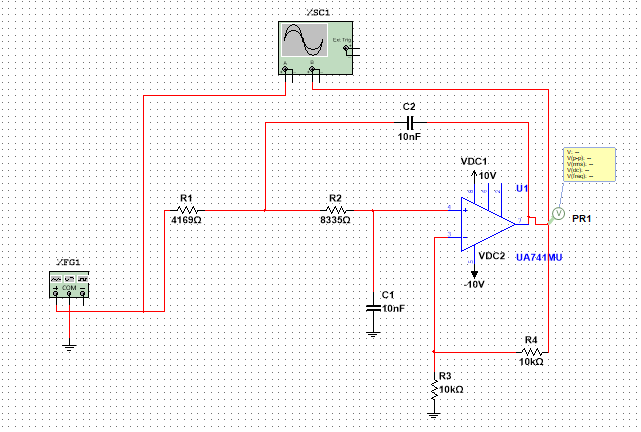
\includegraphics[width=0.8\textwidth]{simulaciones/sallen-montaje.png}
    \caption{Montaje Filtro sallen key}\label{fig:sim-sallen-montaje} 
\end{figure}

\begin{figure}[ht]
    \centering
    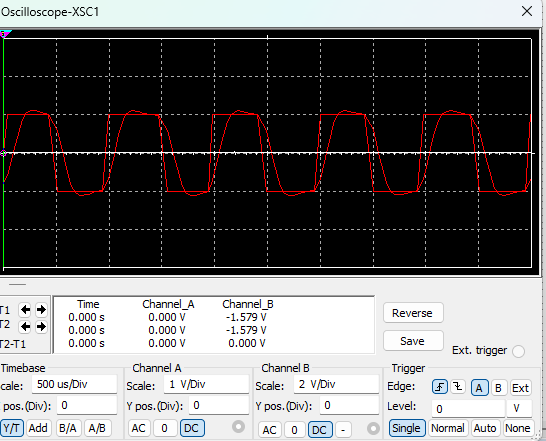
\includegraphics[width=0.8\textwidth]{simulaciones/sallen-cuadrada.png}
    \caption{Filtro sallen key respuesta a onda cuadrada  }
    \label{fig:sim-sallen-cuadrada} 
\end{figure}

\begin{figure}[ht]
    \centering
    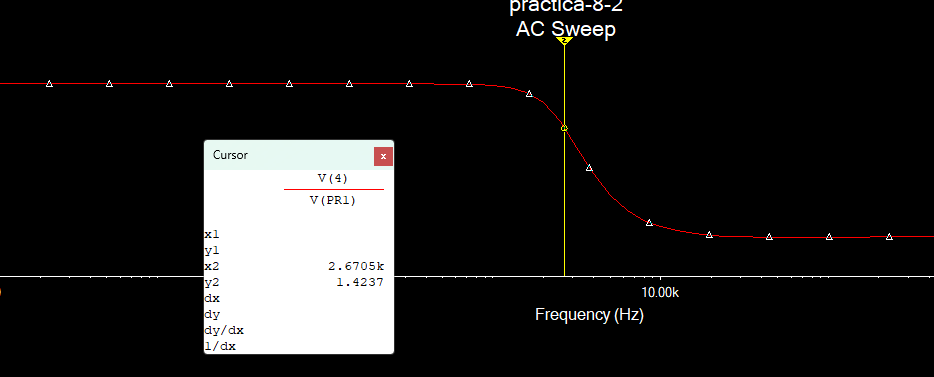
\includegraphics[width=0.8\textwidth]{simulaciones/sallen-respuesta.png}
    \caption{Filtro Sallen key respuesta en frecuencia  }
\end{figure}

\FloatBarrier
\subsubsection{Filtro pasa bajos con realimentación múltiple}

Partiendo de la ecuación \ref{eq:func-transferencia-pasa-bajos-multirealimentacion} de la función de transferencia de un filtro pasa bajos con realimentación múltiple podemos obtener:

\begin{align*}
    H_0 &= \frac{-R_4}{R_1} \\
    R_4 &= - H_0 R_1 \\
\end{align*}

\begin{equation}
    R_4 = 2 R_1\\
    \label{eq:r4-multirealimentacion-pasa-bajos}
\end{equation}

también tenemos que: 

\begin{equation}
    \omega_0 = \sqrt{\frac{1}{R_3 R_4 C_2 C_5}}
    \label{eq:omega-0-multirealimentacion-pasa-bajos}
\end{equation}

Si decimos que: 

\begin{equation*}
    \boxed{C_5 = C_2 = 10nF}
\end{equation*}

la ecuación \ref{eq:omega-0-multirealimentacion-pasa-bajos} se simplifica a:

\begin{equation}
    \omega_0 = \frac{1}{C_2\sqrt{R_3 R_4}}
    \label{eq:omega-0-multirealimentacion-pasa-bajos-simple}
\end{equation}

Por último, tenemos la ecuación:

\begin{equation}
    2\factorAmortiguamiento = \sqrt{\frac{C_5}{C_2}} \left( \sqrt{\frac{R_3}{R_4}} + \sqrt{\frac{R_4}{R_3}} + \frac{\sqrt{R_3 R_4}}{R_1} \right)
    \label{eq:factor-amortiguamiento-multirealimentacion-pasa-bajos}
\end{equation}


que al decir $C_5 = C_2$ entonces la ecuación \ref{eq:factor-amortiguamiento-multirealimentacion-pasa-bajos} se simplifica a:

\begin{equation}
    2\factorAmortiguamiento = \sqrt{\frac{R_3}{R_4}} + \sqrt{\frac{R_4}{R_3}} + \frac{\sqrt{R_3 R_4}}{R_1} 
    \label{eq:factor-amortiguamiento-multirealimentacion-pasa-bajos-simple}
\end{equation}

Ahora, usando la ecuación \ref{eq:omega-0-multirealimentacion-pasa-bajos-simple} en la ecuación \ref{eq:factor-amortiguamiento-multirealimentacion-pasa-bajos-simple} obtenemos:

\begin{equation}
    2\factorAmortiguamiento = \frac{1}{\freqCorte C_2 R_4} + \frac{\freqCorte C_2 R_4}{1} + \frac{1}{\freqCorte R_1 C_2} 
    \label{eq:factor-amortiguamiento-multirealimentacion-pasa-bajos-final}
\end{equation}

Usando \ref{eq:r4-multirealimentacion-pasa-bajos} en la ecuación \ref{eq:factor-amortiguamiento-multirealimentacion-pasa-bajos-final} obtenemos:

\begin{equation}
    2\factorAmortiguamiento = \frac{1}{\freqCorte C_2 2R_1} + \frac{\freqCorte C_2 2R_1}{1} + \frac{1}{\freqCorte R_1 C_2} 
    \label{eq:factor-amortiguamiento-multirealimentacion-pasa-bajos-final-final}
\end{equation}

Todo esto da como resultado:

\begin{align*}
    R_1 &= 1.27k \\
    R_3 &= 640 \\
    R_4 &= 1.88k \\
    C_2 &= 10nF \\
    C_5 &= 100nF \\
\end{align*}

\begin{figure}[ht]
    \centering
    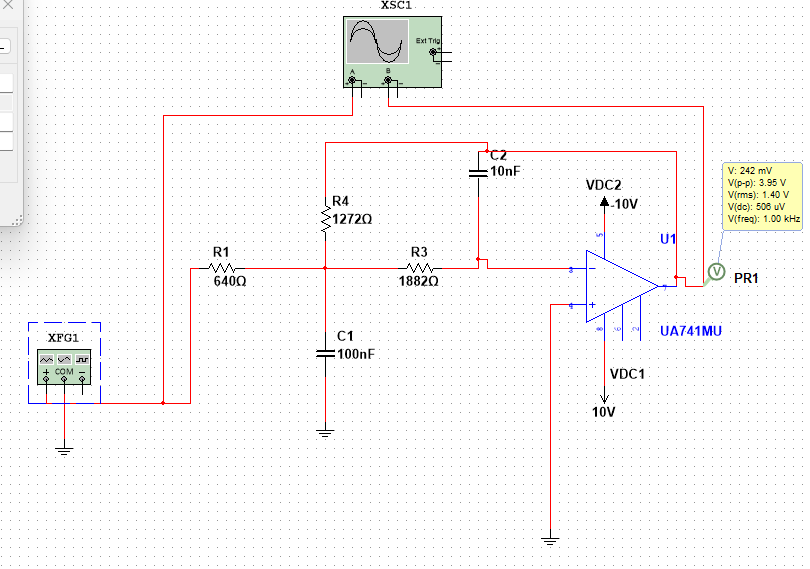
\includegraphics[width=0.8\textwidth]{simulaciones/multirealimentacion-montaje.png}
    \caption{Montaje Filtro multiple realimentación}\label{fig:sim-multirealimentacion-montaje} 
\end{figure}
\begin{figure}[ht]
    \centering
    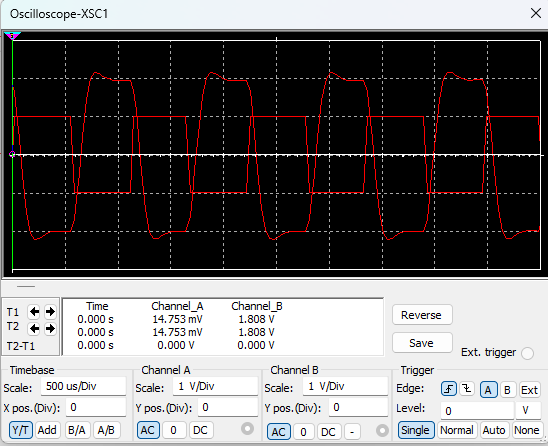
\includegraphics[width=0.8\textwidth]{simulaciones/multirealimentacion-cuadrada.png}
    \caption{Filtro multiple realimentación respuesta a onda cuadrada}
    \label{fig:sim-multirealimentacion-cuadrada} 
\end{figure}
\begin{figure}[ht]
    \centering
    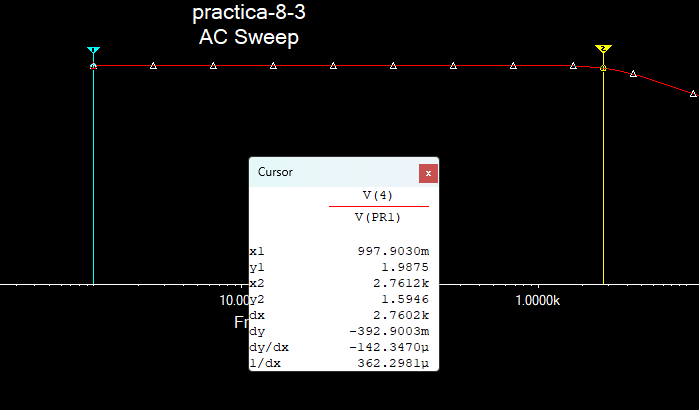
\includegraphics[width=0.8\textwidth]{simulaciones/multirealimentacion-respuesta.png}
    \caption{Filtro multiple realimentación respuesta en frecuencia  }
    \label{fig:sim-multirealimentacion-respuesta} 
\end{figure}

\FloatBarrier
\section{Metodología}

\begin{enumerate}
    \item se monta el circuito de la figura \ref{fig:topologias-basicas} y se energiza con los voltajes $V_{cc}$ y $V_{ee}$. 
    \item Se conecta un generador de señales senoidales y se le conecta un divisor de tensión para obtener dos salidas de voltaje con la misma fase.
    \item  se realiza la conexión del amplificador inversor y se realizan las mediciones de voltaje de entrada $V_i$ y voltaje de salida $V_o$.
    \item se repite el procedimiento anterior para las conexión del amplificador no inversor.
    \item se realizan las conexiones del restador y se toman las medidas de voltaje de entrada $V_1$ y $V_2$ y de salida $V_o$.
    \item se conecta la fuente de corriente con una resistencia $R5$ inicial y se mide la tensión $V_5$ en dicha resistencia, luego se intercambia la resistencia $R5$ por otras resistencias de otros valores y se vuelve a medir el voltaje cada vez.
    \item se cambia el generador para entregar una señal cuadrada, y se realiza la conexión del integrador, conectando el osciloscopio a la salida se ajusta la frecuancia hasta obtener una señal triangular.
\end{enumerate}

\end{document}
